% Options for packages loaded elsewhere
\PassOptionsToPackage{unicode}{hyperref}
\PassOptionsToPackage{hyphens}{url}
%
\documentclass[
]{article}
\usepackage{lmodern}
\usepackage{amssymb,amsmath}
\usepackage{ifxetex,ifluatex}
\ifnum 0\ifxetex 1\fi\ifluatex 1\fi=0 % if pdftex
  \usepackage[T1]{fontenc}
  \usepackage[utf8]{inputenc}
  \usepackage{textcomp} % provide euro and other symbols
\else % if luatex or xetex
  \usepackage{unicode-math}
  \defaultfontfeatures{Scale=MatchLowercase}
  \defaultfontfeatures[\rmfamily]{Ligatures=TeX,Scale=1}
\fi
% Use upquote if available, for straight quotes in verbatim environments
\IfFileExists{upquote.sty}{\usepackage{upquote}}{}
\IfFileExists{microtype.sty}{% use microtype if available
  \usepackage[]{microtype}
  \UseMicrotypeSet[protrusion]{basicmath} % disable protrusion for tt fonts
}{}
\makeatletter
\@ifundefined{KOMAClassName}{% if non-KOMA class
  \IfFileExists{parskip.sty}{%
    \usepackage{parskip}
  }{% else
    \setlength{\parindent}{0pt}
    \setlength{\parskip}{6pt plus 2pt minus 1pt}}
}{% if KOMA class
  \KOMAoptions{parskip=half}}
\makeatother
\usepackage{xcolor}
\IfFileExists{xurl.sty}{\usepackage{xurl}}{} % add URL line breaks if available
\IfFileExists{bookmark.sty}{\usepackage{bookmark}}{\usepackage{hyperref}}
\hypersetup{
  pdftitle={Validating morphological condition indices and their relationship with reproductive success in great-tailed grackles},
  pdfauthor={Berens JM1; Folsom M2; Sevchik A1; Bergeron L3; Logan CJ2; McCune KB3*},
  hidelinks,
  pdfcreator={LaTeX via pandoc}}
\urlstyle{same} % disable monospaced font for URLs
\usepackage[margin=1in]{geometry}
\usepackage{graphicx,grffile}
\makeatletter
\def\maxwidth{\ifdim\Gin@nat@width>\linewidth\linewidth\else\Gin@nat@width\fi}
\def\maxheight{\ifdim\Gin@nat@height>\textheight\textheight\else\Gin@nat@height\fi}
\makeatother
% Scale images if necessary, so that they will not overflow the page
% margins by default, and it is still possible to overwrite the defaults
% using explicit options in \includegraphics[width, height, ...]{}
\setkeys{Gin}{width=\maxwidth,height=\maxheight,keepaspectratio}
% Set default figure placement to htbp
\makeatletter
\def\fps@figure{htbp}
\makeatother
\setlength{\emergencystretch}{3em} % prevent overfull lines
\providecommand{\tightlist}{%
  \setlength{\itemsep}{0pt}\setlength{\parskip}{0pt}}
\setcounter{secnumdepth}{-\maxdimen} % remove section numbering
\usepackage[left]{lineno}
\linenumbers
\usepackage{booktabs}
\usepackage{longtable}
\usepackage{array}
\usepackage{multirow}
\usepackage{wrapfig}
\usepackage{float}
\usepackage{colortbl}
\usepackage{pdflscape}
\usepackage{tabu}
\usepackage{threeparttable}
\usepackage{threeparttablex}
\usepackage[normalem]{ulem}
\usepackage{makecell}
\usepackage{xcolor}

\title{Validating morphological condition indices and their relationship with
reproductive success in great-tailed grackles}
\author{Berens JM\textsuperscript{1} \and Folsom M\textsuperscript{2} \and Sevchik A\textsuperscript{1} \and Bergeron L\textsuperscript{3} \and \href{http://CorinaLogan.com}{Logan CJ}\textsuperscript{2} \and \href{https://www.kelseymccune.com/}{McCune KB}\textsuperscript{3}*}
\date{2020-11-13}

\begin{document}
\maketitle

\hypertarget{affiliations}{%
\subparagraph{Affiliations:}\label{affiliations}}

\begin{enumerate}
\def\labelenumi{\arabic{enumi})}
\tightlist
\item
  Arizona State University School of Life Sciences
\item
  Max Planck Institute for Evolutionary Anthropology
\item
  University of California Santa Barbara
\end{enumerate}

*Corresponding author: KB McCune
(\href{mailto:kelseybmccune@gmail.com}{\nolinkurl{kelseybmccune@gmail.com}})

\textbf{Cite as:} Berens JM, Folsom M, Sevchik A, Bergeron L, Logan CJ,
McCune KB. Submitted to PCI Ecology Nov 2020.
\href{http://corinalogan.com/Preregistrations/gcondition.html}{Validating
morphological condition indices and their relationship with reproductive
success in great-tailed grackles}.

\textbf{This preregistration has been pre-study peer reviewed and
received an In Principle Acceptance by:}

Marcos Mendez (2019 In Principle Acceptance) Are condition indices
positively related to each other and to fitness?: a test with grackles.
\emph{Peer Community in Ecology}, 100035.
\href{https://doi.org/10.24072/pci.ecology.100035}{10.24072/pci.ecology.100035}

\begin{itemize}
\tightlist
\item
  Reviewers: Javier Seoane and Isabel López-Rull
\end{itemize}

\hypertarget{abstract}{%
\subsubsection{ABSTRACT}\label{abstract}}

Morphological variation among individuals has the potential to influence
multiple life history characteristics such as dispersal, migration,
reproductive success, and survival (Wilder et al. 2016). Individuals
that are in better ``condition'' can disperse or migrate further or more
successfully, have greater reproductive success, and survive longer
(Heidinger et al. 2010; Liao et al. 2011; Wilder et al. 2016),
particularly in years where environmental conditions are harsh
(Milenkaya et al. 2015). Body condition is defined in various ways, but
is most often measured using an individual's energetic or immune state
(Milenkaya et al. 2015). These traits are difficult to measure directly,
therefore a variety of morphological proxies to quantify condition are
used instead, including fat score (Kaiser 1993), weight, ratio of weight
to tarsus length (Labocha et al. 2014), a scaled mass index (Peig and
Green 2009), as well as hematological indices for immune system function
(Fleskes et al. 2017; Kraft et al. 2019). However, there is mixed
support regarding whether these condition indices relate to life history
characteristics (Labocha et al. 2014; Wilder et al. 2016), and whether
the relationship is linear (McNamara et al. 2005; Milenkaya et al.
2015). Additionally, although some investigations use multiple
morphological proxies for condition (e.g.~Warnock and Bishop 1998),
rarely have there been direct comparisons among proxies to validate that
they measure the same trait. In this investigation, we define condition
as an energetic state and we attempt to measure it by comparing two
indices (fat score and the scaled mass index) to validate whether they
measure the same trait and whether they correlate with measures of
reproductive success in our study system, the great-tailed grackle
(\emph{Quiscalus mexicanus}). We found that the morphological proxies
did not correlate with each other, indicating that they do not measure
the same trait. Further, neither proxy correlated with reproductive
success in males, measured as whether a male held a territory containing
nests or not. We found that females with a high scaled mass index had a
significantly lower probability that their nest would survive on any
given day. However, there was no relationship between female fat score
and nest survival. These results indicate that measures of condition
should be validated before relying on their use as a condition proxy in
grackles and birds in general. Future research should further
investigate our unexpected result that higher scaled mass index
correlated with lower nest survival to better understand the importance
of energetic condition for reproductive success - a necessary component
for selection to act.

\hypertarget{introduction}{%
\subsubsection{INTRODUCTION}\label{introduction}}

Morphological variation among individuals has the potential to influence
multiple life history characteristics such as dispersal, migration,
reproductive fitness, and survival (Wilder et al. 2016). One
morphological trait that might be particularly likely to influence these
life history characteristics is energetic condition. Individuals that
are in better ``condition'' can disperse or migrate further or more
successfully, have greater reproductive success, and survive longer
(Heidinger et al. 2010; Liao et al. 2011; Wilder et al. 2016),
particularly in years where environmental conditions are harsh
(Milenkaya et al. 2015). For example, a study conducted on vipers showed
that while the level of fat reserves in males was not related to their
sexual activity, females with low fat reserves engaged in sexual
interactions less frequently than those with higher fat reserves (Aubret
et al. 2002). In contrast, mantids showed conflicting results regarding
the relationship between fat reserves and reproductive success (Barry
and Wilder 2013). Female mantids were fed either a high protein, low
lipid diet, or a high lipid, low protein diet. The females that received
the high lipid diet had higher lipid content in most parts of their body
compared to that of their high protein diet counterparts. However, they
were not able to produce even half as many eggs as the females fed the
high protein, low lipid diet. This led to lower male attraction,
measured by the number of copulation events, thus negatively impacting
further reproductive success.

A variety of morphological proxies have been used to quantify energetic
condition (i.e., fat score, weight, ratio of weight to tarsus length,
ratio of weight to wing chord length; Labocha et al. 2014). However,
there is mixed support regarding whether and how these proxies relate to
life history characteristics (Labocha et al. 2014; Wilder et al. 2016).
A review conducted by Barnett (2015) shows that, while mass or body size
measures of condition are often assumed to have a positive linear
relationship with fitness, this is not always the case, and the
relationship should first be empirically validated before being used as
a proxy (Barnett et al. 2015). In some instances, the condition proxy
might relate to life history characteristics, but in an unexpected way.
For example, theoretical simulations of small birds show that survival
does not increase linearly with energy (i.e., fat) reserves (McNamara et
al. 2005). If the reserves are too low, the individual is at risk of
starvation. However, once the reserves get too high, the individual is
at an increased risk of predation (McNamara et al. 2005). Thus, fat
reserves can relate to a life history variable (survival), but in a
U-shaped relationship rather than a linear one.

Although some studies use multiple morphological proxies for condition
(e.g., Warnock and Bishop 1998), rarely are these variables directly
compared. Multiple proxies should correlate with each other if they
measure the same trait (energetic condition). Furthermore, there is
still confusion about what trait some proxies actually measure. For
example, a study conducted on two species of crickets showed that three
estimates of body condition based on fat content or on the relationship
between body mass and body length (scaled mass index or ordinary least
squares regression) did not correlate with each other (Kelly et al.
2014), thus indicating that they do not measure the same trait. This is
an example of the jingle fallacy (Block 1995; Carter et al. 2013), where
a single trait label (``condition'') actually encompasses more than one
distinct trait. In this case, two investigations using different proxies
can be conducted on the same research question, using the same species,
but may end up with different results. This is problematic because
inconsistency in results among researchers can result in potentially
misleading interpretations of the impact of variation in morphology in
relation to life history and population variables (Stevenson and Woods
Jr 2006).

Here we compare two indices (fat score and the scaled mass index) of an
individual's energetic state to validate whether they correlate with
each other, which would indicate that they both measure body condition.
Fat score, as described by Kaiser (1993), is a numerical estimate of the
amount of fat visible under the skin (Fig. 1). The score ranges from 0
to 8 depending on the size and appearance of the fat located in the
individual's abdomen and interclavicular depression, with 0 indicating
no visible fat and 8 indicating extensive fat covering the ventral
surface such that no muscle tissue is visible. For example, a score of 1
corresponds to sparse traces of fat visible in the interclavicular
depression and abdomen. This measure is frequently used in birds (Merilä
and Svensson 1997; Erciyas et al. 2010; Cornelius Ruhs et al. 2019), and
is a straightforward, non-invasive method for estimating condition.
However, previous research found that it does not always positively
relate with life history variables. For example, Haas (1998) found no
difference between fat scores in individuals that had successful or
failed nests in American robins and brown thrashers, indicating that fat
score may not explain much of the variation in nest success in some
species. Further research is needed to understand the relationship
between fat score measures and life history characteristics.

In contrast, the scaled mass index (SMI) is more difficult to calculate
than the fat score, but it has become the predominant ratio method for
quantifying energetic condition within and among populations
(Maceda-Veiga et al. 2014; Delciellos et al. 2018; English et al. 2018).
The SMI is an individual's mass scaled by skeletal body size (Peig and
Green 2009). Unlike the common alternative which uses a simple ratio of
tarsus (lower leg) length to body mass, the SMI accounts for the
tendency towards allometric scaling where the relationship between body
mass and structural size increases by a power law (Huxley 1932). When
individuals with different structural body sizes can be standardized to
the population average structural body size, then energetic condition
(the amount of mass not explained by structural body size) can be more
directly compared within and across populations. That is, the SMI
calculates the energetic condition as the mass of an individual relative
to the population by first computing the mass that the individual would
have at the population average of a specific body measurement (e.g.,
tarsus length). Next, structural body size of the individual is
standardized by scaling the individual's structural body length by the
population average of that body measurement, which accounts for
population differences. The SMI is calculated as:
\(Mass_i\left[ \frac{AvgLength_p}{Length_i} \right]^{slope_p}\) where
\(Mass_i\) is each individual's weight in grams, \(Length_i\) is the
value of the chosen measure of structural body length for each bird,
\(AvgLength_p\) is the average structural body length in the population,
and \(slope_p\) is calculated from the standard major axis regression
(which is used to compare variables that were both directly measured and
thus have residual error) of structural body size on mass (Peig and
Green 2009), and is interpreted as the expected change in structural
length for a one unit increase in mass. Therefore, individuals in better
energetic condition (larger weight for their structural body size) will
have a higher SMI compared to individuals in poor condition. Studies
across taxa found that the SMI relates positively to reproductive
success and survival. For example, mallards with a lower SMI had lower
rates of survival compared to their higher SMI counterparts (Champagnon
et al. 2012), while in crimson finches SMI was positively related to the
number of young that survived to independence (Milenkaya et al. 2015).

Our research will determine whether these two indices of energetic
condition measure the same trait, and whether this trait relates to an
important life history characteristic: reproductive success. Measuring
reproductive success in birds involves finding and monitoring nests
(Mayfield 1961). However, nests are usually built in cryptic locations
and parents behave secretly (Gill 1995), thus making it difficult to
quantify the number of eggs and nestlings inside the nest over time.
Additionally, it is difficult and time-consuming to track the survival
of offspring once they leave the nest. Therefore, we will use the
predominant method in this field for quantifying reproductive success:
whether a nest fledged offspring (Mayfield 1961).

Our study system is a population of great-tailed grackles
(\emph{Quiscalus mexicanus}), hereafter ``grackles'', in Tempe, Arizona.
This system is ideal for this investigation because grackles are native
to the tropical climates of Central America (Johnson and Peer 2001), but
have rapidly expanded their geographic range into new areas (Wehtje
2003). Because grackles are a water-associated species, the desert
habitat of Tempe presents physiological challenges that could lead to an
increased likelihood of a tradeoff between survival and reproductive
attempts (Henderson et al. 2017). Deserts are characterized by a
scarcity of water and extreme temperature fluctuations, which require
behavioral and physiological adaptations (Costa 2012). Wide variation in
body condition and reproductive success is possible if grackle
physiology requires more water than is present in the environment, and
some individuals may cope with physiological stress, or find hidden
sources of water, better than others (Henderson et al. 2017).

\includegraphics[width=0.25\textwidth,height=\textheight]{gconditionfig1a.jpg}
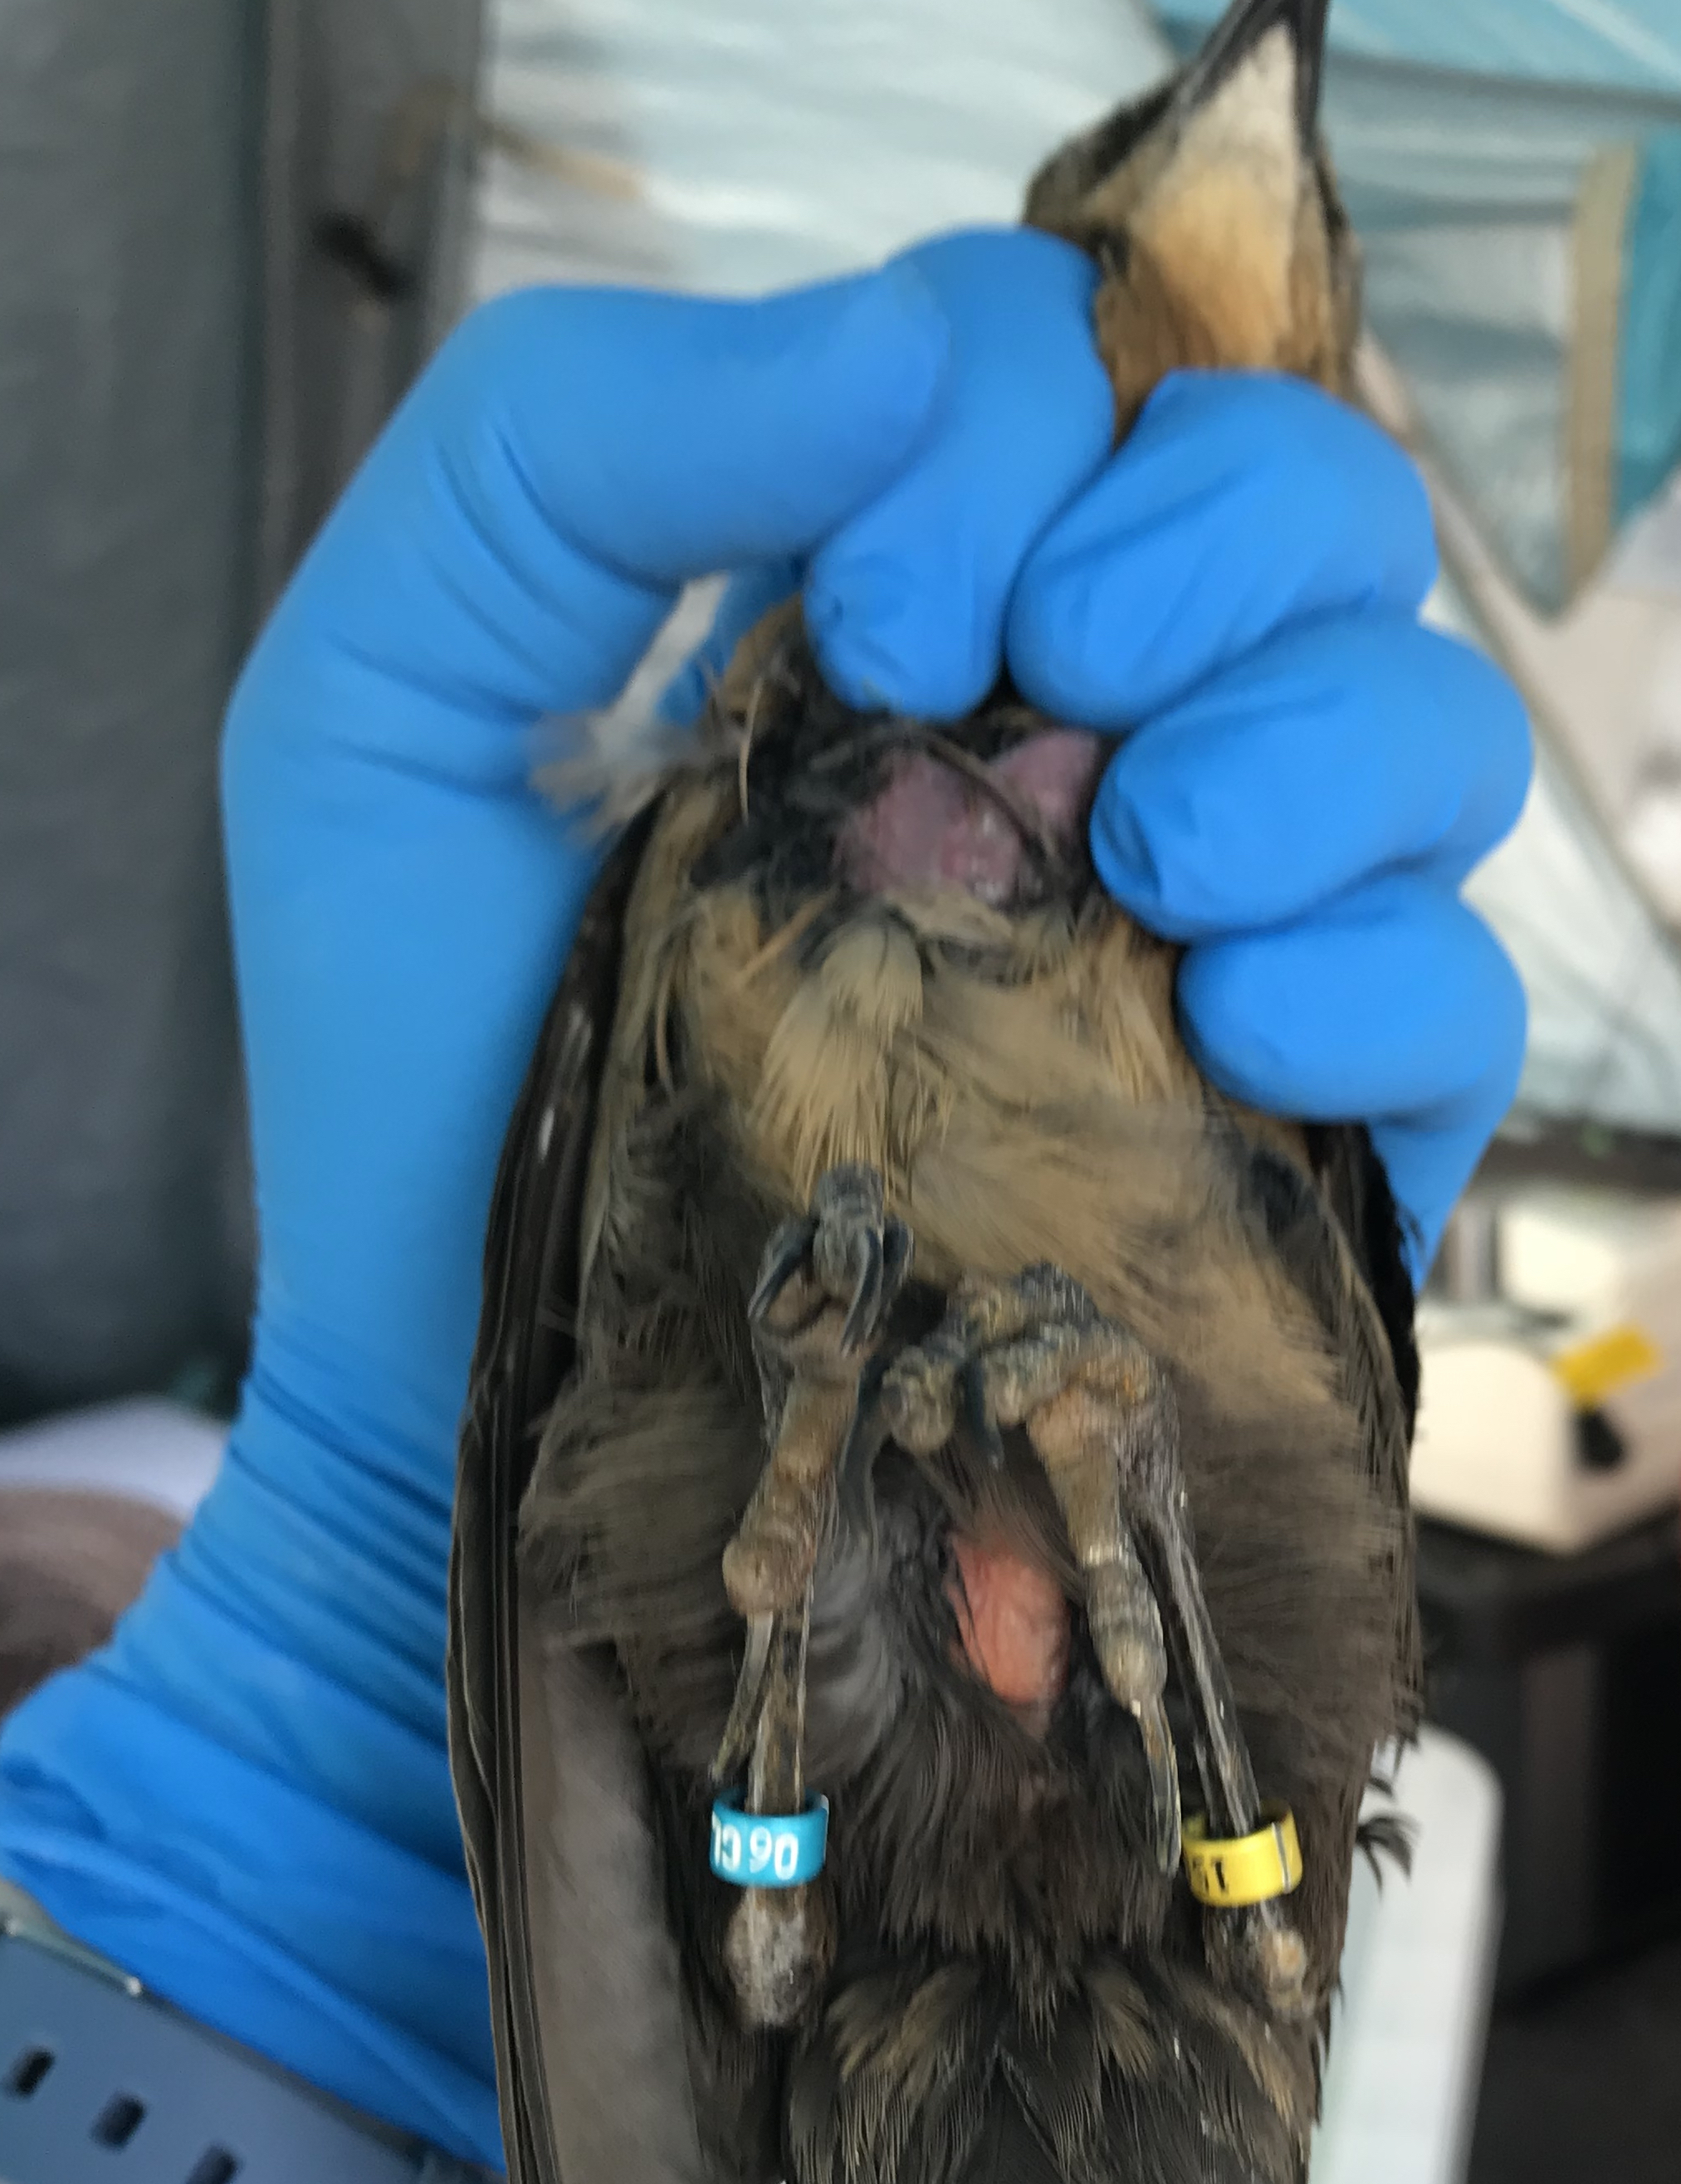
\includegraphics[width=0.25\textwidth,height=\textheight]{gconditionfig1b.jpg}

Figure 1: A male grackle showing the yellow/orange tint of fat under the
skin in the intraclavicular depression (left); and a female grackle
showing \emph{no} fat under the skin of the intraclavicular region, but
significant fat deposits under the skin of the abdomen (right).

\hypertarget{hypotheses}{%
\subsubsection{HYPOTHESES}\label{hypotheses}}

We measured two proxies of body condition and observed reproductive
success in grackles to test two hypotheses:

\textbf{H1 - There is a relationship between two different morphological
indices of condition: fat score and the scaled mass index.}

\textbf{Prediction 1:} Fat score and the scaled mass index will be
positively correlated. This would indicate that these two indices
measure the same trait, and it is likely they both are proxies for fat
content.

\textbf{Prediction 1 alternative 1:} There is a negative correlation
between fat score and the scaled mass index. This would indicate that
there may be a tradeoff between the two indices where a larger value of
the scaled mass index may measure muscle content rather than fat, and
individuals with more muscle have less visible fat.

\textbf{Prediction 1 alternative 2:} There is no correlation between fat
score and the scaled mass index. This indicates that these two variables
do not measure the same trait. Fat score may not adequately capture a
bird's condition because birds may be selected to only store the minimal
fat necessary to prevent starvation, while also minimizing the weight
gain that would make them easier targets for predators (Barnett et al.
2015). Similarly, the scaled mass index could be heavily influenced by
body size, therefore reflecting structural size rather than fat storage
(Labocha and Hayes 2012).

\textbf{H2 - Condition (as measured by fat score and the scaled mass
index) relates to reproductive success (measured as a binary variable of
whether a female had one or more fledglings (1) or not (0), and whether
a male defended a territory containing nests (1) or not (0)).}

\textbf{Prediction 2:} Morphological indices of condition (fat score and
the scaled mass index) will correlate positively with reproductive
success. This would indicate that individuals with more fat, and
therefore higher energy reserves, are better able to acquire the
resources necessary for reproduction.

\textbf{Prediction 2 alternative 1:} Morphological indices of condition
(fat score and the scaled mass index) will correlate negatively with
reproductive success. This indicates that individuals may make trade
offs, with some acquiring more food and increasing their energy
reserves, and others prioritizing reproductive activities over
increasing energy reserves.

\textbf{Prediction 2 alternative 2:} Morphological indices of condition
(fat score and the scaled mass index) do not correlate with reproductive
success. This indicates that other, potentially non-morphological,
individual characteristics relate to reproductive success (i.e.,
cognition, nest site selection, breeding experience, predator vigilance,
etc.).

\hypertarget{associated-preregistration}{%
\subsubsection{ASSOCIATED
PREREGISTRATION}\label{associated-preregistration}}

This preregistration used secondary data that were collected as part of
other ongoing investigations (tarsus length in
\url{http://corinalogan.com/Preregistrations/g_flexgenes.html}; tarsus
length, body weight, number of fledglings, and whether a male holds a
territory in
\url{http://corinalogan.com/Preregistrations/g_withinpop.html}; and
tarsus length in
\url{http://corinalogan.com/Preregistrations/g_expansion.html}). This
preregistration, containing the hypotheses, methods, and analysis plan,
was written (July 2019) and submitted to Peer Community In Ecology for
pre-study peer review (August 2019) before any analyses were conducted.
We revised according to reviewer comments and received in principle
acceptance by PCI Ecology of the version on 8 Nov 2019. After that, we
conducted the analyses in the preregistration. Our final methods,
results, and discussion, including all data and code, are listed below.

\hypertarget{after-pre-study-peer-review-deviations-from-the-planned-methods}{%
\paragraph{\texorpdfstring{\textbf{After pre-study peer review:
Deviations from the planned
methods}}{After pre-study peer review: Deviations from the planned methods}}\label{after-pre-study-peer-review-deviations-from-the-planned-methods}}

\begin{enumerate}
\def\labelenumi{\arabic{enumi})}
\item
  We realized that the sexual dimorphism of male and female body sizes
  necessitates separate analyses. Therefore, we calculated SMI for males
  and females separately, and ran separate models for each sex for the
  repeatibility analysis (P1 and P2).
\item
  Fat score data were distributed such that the majority of scores were
  0, with some 1's and very few higher numbers. This lack of variance in
  the response variable led to problems when we ran the models: it was
  difficult to fit models using an ordinal regression. The function
  ``simulateResiduals'', which we used to check our data, does not work
  with data in the ordinal family. Consequently, we modified the model
  to use a logistic regression where the dependent variable FatScore is
  categorized as individuals that showed no visible fat (y = 0), or some
  fat was present (y = 1) where we combined all individuals that had fat
  score values of 1 or greater. Subsequent data checking indicated that
  these data were not zero-inflated or overdispersed.
\end{enumerate}

\hypertarget{p1-correlation-between-smi-and-fat-score}{%
\subparagraph{P1: correlation between SMI and Fat
score}\label{p1-correlation-between-smi-and-fat-score}}

\begin{enumerate}
\def\labelenumi{\arabic{enumi})}
\setcounter{enumi}{2}
\item
  Warning messages occurred during the repeatability analysis using the
  ``rptR'' package in R (Stoffel et al. 2017) indicating that the fit
  was singular, likely because the variance for the Experimenter random
  effect in the model for both female and male wing length was 0.001. We
  thus conducted an unregistered analysis where we confirmed that our
  repeatability values from the repeatability models were valid, despite
  the warning, by hand calculating repeatability following Nakagawa and
  Schielzeth (2010). The hand-calculated repeatabilities were nearly
  identical (female R = 0.5, male R = 0.71) to the output from the rpt
  function.
\item
  Despite the data checking which indicated our model was not
  overdispersed or zero inflated, we could not get the fixed effects or
  random effect to converge using the Bayesian package in R
  ``MCMCglmm''. We found no improvement in model fit by tweaking the
  priors or iterations/burnin/thin options. Therefore, we fit these
  models using the function glmer, a frequentist framework.
\item
  The Season variable only includes 2 males in the breeding season
  category, thus we do not have a large enough sample to produce
  reliable estimates. We removed the Season variable from the model for
  males.
\end{enumerate}

\hypertarget{p2-body-condition-and-reproductive-success}{%
\subparagraph{P2: body condition and reproductive
success}\label{p2-body-condition-and-reproductive-success}}

\begin{enumerate}
\def\labelenumi{\arabic{enumi})}
\setcounter{enumi}{5}
\item
  Only two females had reproductive success data from more than one year
  in our study (2019 and 2020). Consequently, there were very few
  repeated measures in this sample and our random effect of bird ID
  accounted for zero variance. This led to a warning that our model fit
  was singular. Therefore, we removed the data for these females for
  2020 so we could remove ID as a random effect from the model, which
  resulted in the model running without warnings. We removed the 2020
  data for these females because their condition data was collected in
  2019 and these measures were more likely to relate to their 2019
  reproductive success data than to their reproductive success in 2020.
\item
  The fit of the model analyzing the relationship between body condition
  and male reproductive success (ability to hold a territory containing
  female nests) was singular. The Year random effect accounted for zero
  variance in the data, so we removed it. The fit was still singular,
  but we retained the ID random effect (although it also explained zero
  variance) to account for repeated measures in this sample.
\item
  The model fit was again singular in our logistic exposure model
  because the Year random effect explained zero variance in the data. We
  removed this random effect from the analysis.
\end{enumerate}

\pagebreak

\hypertarget{results}{%
\subsubsection{RESULTS}\label{results}}

\textbf{Prediction 1: correlation between SMI and Fat Score}

We were able to calculate SMI for 24 males and 62 females, and fat score
values were available for 21 males and 47 females.

We found that wing length was more tightly correlated with body mass
than tarsus length in both sexes, therefore we used wing length in our
SMI calculations (female n = 62, r = 0.26, \emph{p} = 0.03; male n = 24,
r = 0.35, \emph{p} = 0.08). This allows us to account for as much
variation in body mass as possible that is associated with skeletal body
size because leftover variation in body mass is more likely to relate to
energetic condition. Consequently, we used wing length in our
calculation of SMI as:
\(Mass_i\left[ \frac{AvgWing_p}{AvgWing_i} \right]^{slope_p}\).
\(Mass_i\) is each individual's weight in grams, \(AvgWing_i\) is the
average value of the measures of the left and right wing lengths of each
bird, \(AvgWing_p\) is the average wing length in the population, and
\(slope_p\) is the value of the slope from a standard major axis
regression of the population's wing length on the population's mass
(Peig and Green 2009).

To validate that we were measuring structural body size consistently
across experimenters, we analyzed the repeatability of wing length in
the birds in our sample that were measured more than once. We found that
average wing length was repeatable (n = 17 females, Repeatability ±
standard error = 0.53 ± 0.18; n = 18 males, Repeatability ± SE = 0.75 ±
0.11). Data permutations and a likelihood ratio test both confirmed that
these repeatability values were statistically significant at p
\textless{} 0.01.

We found that fat score was not correlated with SMI, which indicates
that they are not measuring the same trait (female \emph{p} = 0.81; male
\emph{p} = 0.50; Table 1). There was also no relationship between season
(breeding or non-breeding) and female fat score (\emph{p} = 0.71). Only
2 males were measured during the breeding season, therefore we omitted
season as an independent variable in the male model.

\begin{table}

\caption{\label{tab:p1 results}Table 1. Results from the logistic mixed-effect regression for females and fixed-effect regression for males to determine whether fat score and scaled mass index (SMI) are correlated. Estimates are presented with the standard error in parentheses. Our sample size was too small to test for a season effect in males.}
\centering
\begin{tabular}[t]{l|c|c|c|c}
\hline
\multicolumn{1}{c|}{ } & \multicolumn{2}{c|}{Females} & \multicolumn{2}{c}{Males} \\
\cline{2-3} \cline{4-5}
Parameter & Estimate (SE) & p-value & Estimate (SE) & p-value\\
\hline
Intercept & -0.20 (0.74) & 0.79 & -0.82 (0.64) & 0.21\\
\hline
SMI & 0.07 (0.30) & 0.81 & 0.46 (0.62) & 0.46\\
\hline
Season & 0.27 (0.71) & 0.70 & NA & NA\\
\hline
\end{tabular}
\end{table}

\textbf{P2: body condition and reproductive success}

Our sample size for P2, where individuals had measures of reproductive
success, SMI, and fat scores, was 20 for females and 20 for males.

In some investigations, body condition shows a non-linear relationship
with reproductive success (Milenkaya et al. 2015). To test for this, we
calculated the SMI categories using 0.5 standard deviation (sd)
increments around the mean to determine whether individuals in some
categories were more likely to be reproductively successful. Category 1
is ``low'' SMI and includes birds with SMI values that are more than 1
sd less than the mean, category 2 is ``moderately low and ranges from
0.5 sd to 1 sd less than the mean, category 3 is''moderate" and includes
individuals with SMI values between 0.5 less than the mean and 0.5 sd
greater than the mean, category 4 includes individuals with SMI values
between 0.5 and 1 sd greater than the mean and category 5 includes
individuals with SMI values that are more than 1 sd greater than the
mean. However, we found no evidence for a non-linear relationship
between reproductive success and SMI for males or females (Fig. 2).

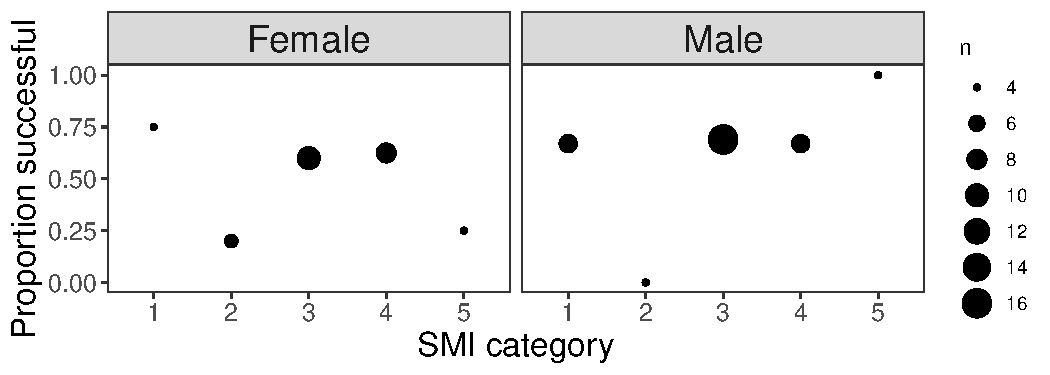
\includegraphics{gcondition_files/figure-latex/p2 non-linear trend results-1.pdf}

Figure 2: The proportion of individuals that successfully fledged nests
(females: left) or held a territory (males: right) in low (1),
moderately low (2), moderate (3), moderately high (4) and high (5)
scaled mass index (SMI) categories. Dots are sized according to the
number (n) of individuals in that category. There is no evidence of a
non-linear relationship.

We used linear models to determine whether season would be important to
include in our models testing P2. We found that neither SMI (female
\emph{p} = 0.26, male \emph{p} = 0.15) nor fat score (female \emph{p} =
0.68, male \emph{p} = 0.99) differed by season in females or males (Fig.
3). Although we note that, as stated above, we lack sufficient fat score
data from males in the breeding season so results from that model should
be interpreted with caution. Consequently, we did not include season as
an independent variable in the P2 models.

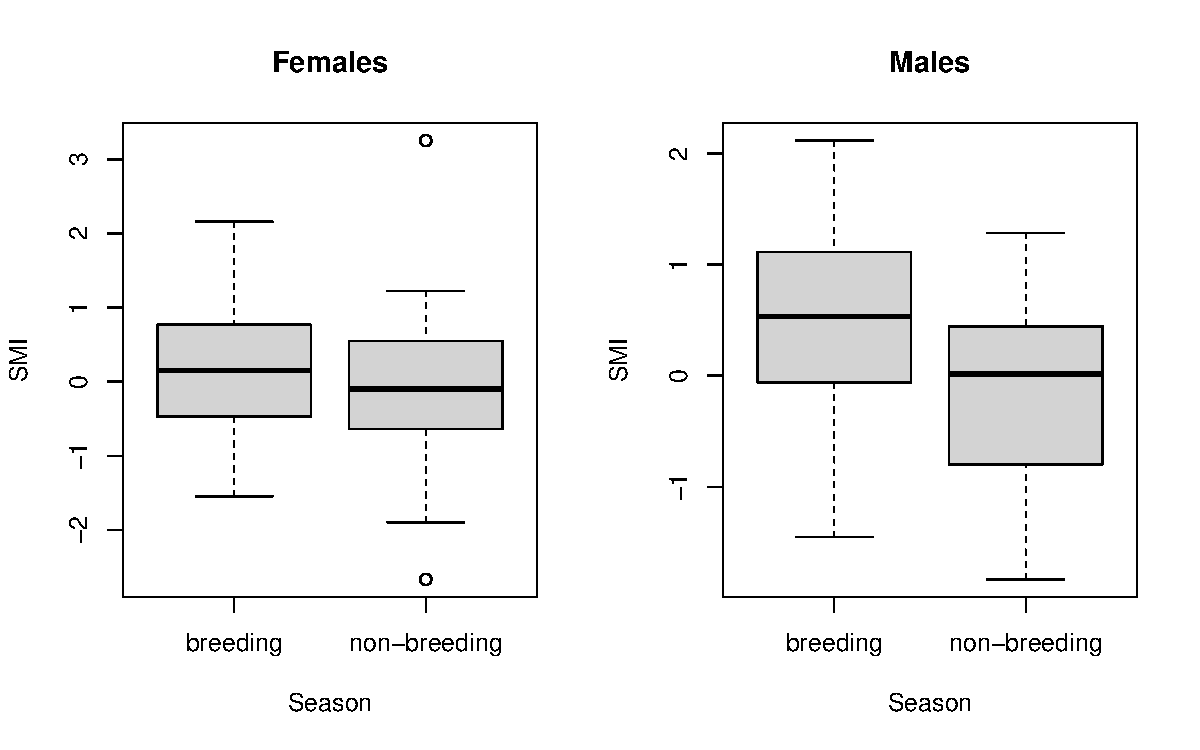
\includegraphics{gcondition_files/figure-latex/p2 condition and season-1.pdf}

Figure 3: Scaled mass index (SMI) was not significantly different
between the breeding and non-breeding seasons for either sex.

Because fat score and SMI did not correlate, we included both as
independent variables in our models testing prediction 2. We found that
neither SMI (\emph{p} = 0.13), nor fat score (\emph{p} = 0.82) was
associated with whether a female fledged offspring (Table 2). There was
also no evidence of a relationship between the ability of a female to
produce fledglings and having previously spent time in the aviaries
(\emph{p} = 0.22). For males, the ability to defend a territory was also
unrelated to either SMI (\emph{p} = 0.13) or fat score (\emph{p} =
0.76). Additionally, we found that those males who spent more time in
the aviaries were less likely to hold a territory compared with males
who were never in the aviaries or who spent less time in the aviaries
(\emph{p} = 0.02). However, we stress that our sample size was
relatively small (20 males), and we did not have a balanced sample
because there were no males that did not defend a territory and were
never in the aviaries. Additionally, only five males had data from more
than one breeding season, which resulted in our model fit being singular
because the random effect for bird ID accounted for essentially zero
variance. However, we kept ID in the model to account for the repeated
samples.

\begin{table}

\caption{\label{tab:p2 main results}Table 2. Results from the logistic regression for females and males to test whether reproductive success relates to condition. Estimates are presented with the standard error in parentheses.}
\centering
\begin{tabular}[t]{l|c|c|c|c}
\hline
\multicolumn{1}{c|}{ } & \multicolumn{2}{c|}{Females} & \multicolumn{2}{c}{Males} \\
\cline{2-3} \cline{4-5}
Parameter & Estimate (SE) & p-value & Estimate (SE) & p-value\\
\hline
Intercept & -0.02 (0.73) & 0.98 & 3.05 (1.40) & 0.03\\
\hline
FatScore & 0.15 (1.02) & 0.89 & -0.33 (1.10) & 0.77\\
\hline
SMI & -0.92 (0.61) & 0.13 & 1.18 (0.78) & 0.13\\
\hline
Aviary & -1.38 (1.14) & 0.23 & -3.62 (1.56) & 0.02\\
\hline
\end{tabular}
\end{table}

\pagebreak

\textbf{P2: body condition and probability of daily nest survival}

Logistic regression analyses to determine reproductive success from
nests discovered in different stages will be systematically biased
(Shaffer 2004). Nests discovered at a more progressed stage (i.e.,
nestling stage compared to building stage) are statistically more likely
to succeed and nests with frequent and prolonged adult visits (such as
those that occur when nests survive longer) are more likely to be
discovered. Therefore, nests that fail early are less likely to be
detected (Shaffer 2004). Consequently, we analyzed female reproductive
success using a logistic exposure model (Bolker 2014), which uses
survival analysis to determine the factors affecting the probability of
daily nest survival, while accounting for incomplete nest observations.
We found that the probability of daily nest survival was significantly
negatively related to SMI (\emph{p} = 0.03; Table 3), where, for every
unit increase in SMI, the odds of daily nest survival decreased by half.
This indicates that a female with a larger SMI (more mass for her
structural body size) was less likely to have her nest survive each day
(Fig. 4). There was no statistically significant relationship between
the probability of daily nest survival and fat score, day of the year,
or time spent in the aviaries (Table 3). Although not statistically
significant, the effect size for the relationship between fat score and
daily nest survival is large (Fig. 4) and potentially biologically
meaningful. The odds of a nest surviving on a given day are almost 2.5
times greater for birds with some fat (a score of 1) compared to no fat
(a score of 0).

\textbackslash begin\{table\}

\textbackslash caption\{\label{tab:logexp}Table 3. Results of the
logistic exposure model showing the relationship between the probability
of daily nest survival and scaled mass index (SMI), fat score, the
amount of time spent in the aviaries, and the day of the year. Odds
ratios (OR) are the exponentiated estimates to increase
interpretability. SE=Standard Error, CI=95\% Confidence Interval\}
\centering

\begin{tabular}[t]{l|c|c|c}
\hline
Parameter & Estimate (SE) & OR (CI) & p-value\\
\hline
Intercept & 1.99 (0.40) & 7.32 (3.3-16.0) & <0.001\\
\hline
Fat score & 0.91 (0.49) & 0.50 (0.27-0.92) & 0.06\\
\hline
SMI & -0.69 (0.31) & 2.48 (0.95-6.49) & 0.03*\\
\hline
Day of year & -0.21 (0.15) & 0.63 (0.19-2.10) & 0.16\\
\hline
Aviary & -0.47 (0.61) & 0.81 (0.60-1.10) & 0.44\\
\hline
\end{tabular}

\textbackslash end\{table\}

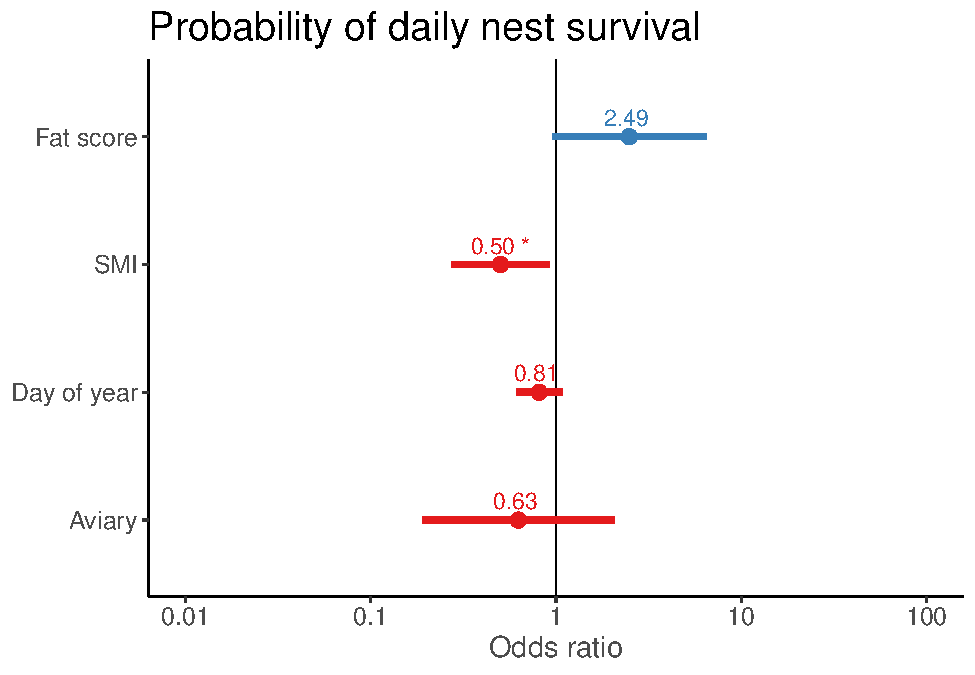
\includegraphics{gcondition_files/figure-latex/logexp-1.pdf} Figure 4.
Odds ratios for independent variables affecting the probability of a
nest surviving a given day. The dots and corresponding values represent
the odds ratio values, and lines represent the confidence intervals
around the odds ratio value. The vertical line at x = 1 delineates the
odds ratio value for no relationship between the estimates and the
probability of daily nest survival. The asterisk indicates an odds ratio
value that is statistically significant.

\hypertarget{discussion}{%
\subsubsection{DISCUSSION}\label{discussion}}

Although it is often implicitly assumed that most condition proxies
measure the same trait, we found that two proxies of energetic
condition, fat score and SMI, did not correlate with each other in the
great-tailed grackle, regardless of whether it was the breeding or
non-breeding season. Further, we found that neither fat score nor SMI
correlated with a female's ability to produce fledglings or a male's
ability to hold a territory containing nests. However, we did find that
the probability a female's nest will survive a given day is negatively
related to SMI. These results have implications for the interpretation
of results that are based on such proxies and for the use of these
proxies in future research.

There are several potential reasons why grackle fat score and SMI did
not correlate. First, it is possible that we were unable to accurately
measure the amount of fat the birds actually stored. In addition to
storing fat under their skin, birds may also store fat intraperitoneally
(Musacchia 1953), which would not have been detected with our fat score
measure. Second, variation in mass among grackles might have resulted
from not only variation in fat content, but also from variation in
muscle content (Labocha and Hayes 2012). However, measuring muscle
content requires destructive methods (i.e.~sacrificing the birds; Zhang
et al. 2015), which was beyond the scope of the current research
program. Third, it is possible that fat score and SMI did not correlate
due to experimenter error in collecting these measurements. We were
unable to quantify the repeatability of our measures within and between
experimenters because we did not collect repeated measurements on the
same grackles when they were in hand (to reduce the amount of processing
time a bird experiences). Finally, our sample size might have been too
small to detect an effect. However, the effect size for the relationship
between fat score and SMI was essentially zero (0.001), therefore it is
unlikely that a larger sample size would find a biologically informative
relationship between these two proxies.

Although our first analysis of reproductive success, measured as the
ability to produce fledglings (females) or to hold a territory
containing nests (males), found no correlation with fat score or SMI,
when we used logistic exposure models to determine whether female body
condition related to the probability of daily nest survival, we found a
negative relationship between SMI and the likelihood of daily nest
survival. This result was surprising, but could be due to larger females
actually carrying proportionally smaller energetic reserves than their
smaller female counterparts, as seen in red-winged blackbirds (Langston
et al. 1990). In some species, females with smaller body sizes are able
to initiate breeding earlier because they can allocate more resources to
reproduction compared to larger individuals that have higher bodily
energy demands and therefore fewer excess energetic resources (Murphy
1986; Langston et al. 1990; Barbraud et al. 2000). This indirectly
affects reproductive success because nesting earlier increases the
probability of nesting success and multiple nesting attempts (Perrins
1970; Johnson and Peer 2001). Yet, we found no relationship between the
probability of daily nest survival and day of the year, therefore this
is unlikely to explain the negative relationship between SMI and nest
survival. Alternatively, it is possible that larger females are unable
to build a more concealed nest in the most dense vegetation, or that
larger females are more likely to disrupt nest stability. The grackle
nests were very high (often \textgreater10m above ground) and usually
fairly well concealed, so we could not determine the causes of nest
failure. Further investigations would be required to determine how body
condition relates to specific threats to nesting success. In addition,
the parameter estimate for the relationship between fat score and the
daily probability of nest survival indicates that females with some
visible fat are more than twice as likely to have a nest survive a given
day. Because the direction of this effect is opposite to the
relationship between SMI and nest survival, this is further evidence
that these two proxies represent different traits, and that SMI is
likely influenced by muscle mass.

Measurements of energetic condition are important for understanding
variation in life history characteristics in studies across the animal
kingdom. However, the results of this study highlight the need to better
understand proxy measures of condition, not only in grackles, but for
birds in general. Most studies on avian energetic condition only use one
proxy for condition, but because energetic condition is difficult to
measure directly, it is important to compare multiple proxy variables to
ensure each proxy is measuring the intended trait (the jingle-jangle
fallacy; Block 1995; Carter et al. 2013). Future research could add to
this work by incorporating additional methods to measure energetic
condition, for example, blood hematocrit levels (Dawson and Bortolotti
1997), protein storage (Houston et al. 1995), or by studying additional
traits that could relate to variation in energy stores, such as
dispersal (Ellers et al. 1998) or survival (Liao et al. 2011).
Furthermore, future research would benefit from using logistic exposure
models to examine the relationship between body condition and
reproductive success because these models control for the bias that
arises when early nest failures are not detected, which is not possible
in logistic regression models, and it is more sensitive to changes in a
bird's nest status (Shaffer 2004).

\pagebreak

\hypertarget{methods}{%
\subsubsection{METHODS}\label{methods}}

The methods below are based on the preregistration, with small changes
as described in the
\protect\hyperlink{associated-preregistration}{Deviations from the
preregistration} section above.

\hypertarget{planned-sample}{%
\paragraph{\texorpdfstring{\textbf{Planned
Sample}}{Planned Sample}}\label{planned-sample}}

Great-tailed grackles are caught in the wild in Tempe, Arizona using a
variety of methods (e.g., walk-in trap, bownet, mist net). After capture
we immediately process birds by attaching colored leg bands in unique
combinations for individual identification, conducting morphological
measurements of weight, tarsus length, flattened wing length, tail
length, skull length, bill length and fat score (the amount of visible
fat under the skin in the clavicle and abdomen as in Kaiser 1993). Most
grackles are released after completion of color band marking,
measurements, and acquiring a blood sample. A subset of grackles are
held in aviaries for up to 6 months for behavioral testing, and then
released back to the wild at their location of capture.

From March - August, we monitor the behavior of all color-marked
grackles to determine their nesting status. We follow females carrying
nesting materials to find their nest. We determine whether the male
territory owner is color-marked as well. Then we check each nest
approximately every day to determine the status based on the female's
behavior (building, incubation, feeding nestlings, feeding fledglings,
failed).

Individuals included in this sample will be those for which we have
measures of condition when they were adults. We will not include
individuals whose data were collected as juveniles. As of 30 July 2019,
we have fledgling data for 14 females that exhibited breeding behavior
(5 had 1+ fledgling, 9 had no fledglings) and breeding territory status
for 10 males (7 territory holders, 3 non-territory holders, 2 not
observed so not part of this sample). Therefore, the minimum sample size
for H2 will be 24. The minimum sample size for H1 will be 72, because
that is how many marked individuals we have biometric data for so far.
However, we expect to be able to add to the sample size for both H1 and
H2 before the end of this investigation in Tempe, Arizona. \emph{UPDATE
Oct 2020: In the second breeding season we had 20 females and 20 males
with reproductive success and body condition data.}

\hypertarget{sample-size-rationale}{%
\paragraph{\texorpdfstring{\textbf{Sample size
rationale}}{Sample size rationale}}\label{sample-size-rationale}}

We will continue to color mark as many grackles as possible, and collect
biometric data and fat scores. Our current sample of reproductive
success is small because the grackles in Tempe nest in very tall palms,
making it difficult to determine nest status. However, we plan to
collect additional reproductive success data during the breeding season
in summer 2020. \emph{UPDATE Oct 2020: In the second breeding season we
had 20 females and 20 males with reproductive success and body condition
data.}

\hypertarget{data-collection-stopping-rule}{%
\paragraph{\texorpdfstring{\textbf{Data collection stopping
rule}}{Data collection stopping rule}}\label{data-collection-stopping-rule}}

We will stop collecting data for this project in early August 2020 when
research at the Tempe, Arizona field site will be finished.

\hypertarget{open-materials}{%
\paragraph{\texorpdfstring{\textbf{Open
materials}}{Open materials}}\label{open-materials}}

Biometric measurement protocol:
\url{https://gitlab.com/corinalogan/the-grackle-project/blob/master/protocolBiometrics.pdf}

Nest check protocol:
\url{https://gitlab.com/corinalogan/the-grackle-project/blob/master/protocolNestCheck.pdf}

\hypertarget{open-data}{%
\paragraph{\texorpdfstring{\textbf{Open
data}}{Open data}}\label{open-data}}

All data (Berens 2020) are available at
\url{https://knb.ecoinformatics.org/view/doi:10.5063/F1NZ862D} and at
github (the provided code will load these files directly from github).

\hypertarget{randomization-and-counterbalancing}{%
\paragraph{\texorpdfstring{\textbf{Randomization and
counterbalancing}}{Randomization and counterbalancing}}\label{randomization-and-counterbalancing}}

There is no randomization or counterbalancing in this investigation.

\hypertarget{blinding-of-conditions-during-analysis}{%
\paragraph{\texorpdfstring{\textbf{Blinding of conditions during
analysis}}{Blinding of conditions during analysis}}\label{blinding-of-conditions-during-analysis}}

No blinding is involved in this investigation.

\textbf{Dependent Variables}

\textbf{P1: correlation between fat and the scaled mass index}

\begin{enumerate}
\def\labelenumi{\arabic{enumi})}
\tightlist
\item
  Fat score (the amount of visible fat under the skin in the clavicle
  and abdomen reported as a score from 0 (no fat) to 8 (fat completely
  covers muscles and underside of the bird); Kaiser 1993) \emph{UPDATE
  Oct 2020: Fat score was heavily 0 skewed with few scores greater than
  one. To increase model fit we used a binomial response variable
  instead, where 0 is no fat and 1 is some fat observed undert the
  skin.}
\end{enumerate}

\textbf{P2: condition and reproductive success}

\begin{enumerate}
\def\labelenumi{\arabic{enumi})}
\item
  Female had one or more fledglings (yes, no)
\item
  Male held a territory consisting of 1 to 3 clumped palms containing
  nests (yes, no)
\end{enumerate}

\textbf{Independent Variables}

\textbf{P1: correlation between fat and the scaled mass index}

\begin{enumerate}
\def\labelenumi{\arabic{enumi})}
\item
  Scaled mass index using measures of body weight and tarsus length or
  flattened wing length (average of left and right as in Bleeker et al.
  2005). We will choose the measure that is most correlated with body
  weight (Peig and Green 2009).
\item
  Season (non-breeding {[}Sep-Feb{]}, breeding {[}Mar-Aug{]}).
  \emph{UPDATE Oct 2020: The Season variable only includes 2 males in
  the breeding season category, thus we do not have a large enough
  sample to produce reliable estimates. We removed the Season variable
  from the model for males.}
\item
  Random effect: Experimenter (because several different experimenters
  measure dependent variables on multiple different birds)
\end{enumerate}

\textbf{P2: condition and reproductive success}

\begin{enumerate}
\def\labelenumi{\arabic{enumi})}
\item
  Fat score

  \begin{itemize}
  \tightlist
  \item
    Note 1: if the fat score and the scaled mass index are positively
    correlated, then we will use only fat score in the model for P2. If
    they are not positively correlated, then we will add the scaled mass
    index as an independent variable in the P2 analysis
  \item
    Note 2: if fat score and/or the scaled mass index vary by season
    (breeding or non-breeding), then we will only use the data from the
    breeding season to ensure that less time has elapsed between the
    collection of condition and reproductive success variables
  \end{itemize}
\item
  Temporarily held in aviaries for behavioral testing at any point
  during this study, because this may affect breeding behaviors (yes,
  no)
\item
  Random effect: Year (to determine whether conditions in a given
  breeding season similarly affected all grackle behavior and nest
  success)
\item
  Random effect: Bird ID (because there may be multiple measures of
  reproductive success for each bird)
\end{enumerate}

\hypertarget{analysis-plan}{%
\subsubsection{ANALYSIS PLAN}\label{analysis-plan}}

\emph{UPDATE Oct 2020:}

\emph{1) We realized that the sexual dimorphism of male and female body
sizes necessitates separate analyses. Therefore, we calculated SMI for
males and females separately, ran separate models for each sex for the
repeatibility analysis, P1 and P2.}

\emph{2) Fat score data were distributed such that the majority of
scores were 0, with some 1's and very few higher numbers. This made it
difficult to fit models using an ordinal regression. The function
simulateResiduals, which we used to check our data, does not work with
data in the ordinal family. Consequently, we used logistic regression
where the dependent variable FatScore represents no fat (score = 0), or
some fat (score = 1)}

\emph{3) Despite the data checking which indicated our model was not
overdispersed or zero inflated, we could not get the fixed effects or
random effect to converge using the Bayesian MCMCglmm. We found no
improvement in model fit by tweaking the priors or
iterations/burnin/thin options. Therefore, we fit these models using the
function glmer, a frequentist framework.}

\emph{4) The Season variable only includes 2 males in the breeding
season category, thus we do not have a large enough sample to produce
reliable estimates. We removed the Season variable from the model for
males.}

We will \textbf{exclude} data that was collected from the grackles when
they were released from the aviaries to avoid any confounds due to their
time in the aviary (e.g., perhaps unlimited nutritious food in the
aviaries decreased their fat score). However, to validate that our
measures of structural body size (tarsus length or wing length) are
precise and accurate, we will measure twice a subset of grackles brought
into aviaries - once when they are initially caught, and again up to 6
months later when we release them. We will then calculate the
repeatability of these multiple measures. All other data included in
this study will come only from wild-caught grackles (including the birds
that were brought into the aviaries on their first capture). When
\textbf{missing data} occur, the existing data for that individual will
be included in the analyses for which their data exist. Analyses will be
conducted in R (current version 4.0.2; R Core Team 2017).

\hypertarget{ability-to-detect-actual-effects}{%
\paragraph{\texorpdfstring{\emph{Ability to detect actual
effects}}{Ability to detect actual effects}}\label{ability-to-detect-actual-effects}}

To begin to understand what kinds of effect sizes we will be able to
detect given our sample size limitations, we used G*Power (v.3.1, Faul
et al. 2007: @faul2009statistical) to conduct power analyses based on
confidence intervals. G*Power uses pre-set drop down menus and we chose
the options that were as close to our analysis methods as possible
(listed in each analysis below). Note that there were no explicit
options for GLMMs, thus the power analyses are only an approximation of
the kinds of effect sizes we can detect. We realize that these power
analyses are not fully aligned with our study design and that these
kinds of analyses are not appropriate for Bayesian statistics (e.g., our
MCMCglmm below), however we are unaware of better options at this time.
Additionally, it is difficult to run power analyses because it is
unclear what kinds of effect sizes we should expect due to the lack of
data on this species for these particular research questions.

\hypertarget{data-checking}{%
\paragraph{\texorpdfstring{\emph{Data
checking}}{Data checking}}\label{data-checking}}

The data will be checked for overdispersion, underdispersion,
zero-inflation, and heteroscedasticity with the DHARMa R package (Hartig
2019) following methods by
\href{https://cran.r-project.org/web/packages/DHARMa/vignettes/DHARMa.html}{Hartig}.

\emph{P1 analysis: correlation between fat and the scaled mass index}

We will calculate the scaled mass index as described by Peig and Green
(2009) using either tarsus or flattened wing length - whichever measure
is most correlated with body weight (Peig and Green 2009).

We use a Generalized Linear Mixed Model (GLMM; MCMCglmm function,
MCMCglmm package; (Hadfield 2010)) with an ordinal distribution (for
categorical variables in MCMCglmm) and probit link using 130,000
iterations with a thinning interval of 10, a burnin of 30,000, and
minimal priors (V=1, nu=0) (Hadfield 2014). We will ensure the GLMM
shows acceptable convergence (lag time autocorrelation values
\textless0.01; Hadfield 2010), and adjust parameters if necessary to
meet this criterion. We will determine whether an independent variable
had an effect or not using the Estimate in the full model.

Where we have multiple measures of tarsus or flattened wing length, we
will check that our measurements are repeatable using the rptR package
(Stoffel et al. 2017).

To roughly estimate our ability to detect actual effects (because these
power analyses are designed for frequentist statistics, not Bayesian
statistics), we ran a power analysis in G*Power with the following
settings: test family=F tests, statistical test=linear multiple
regression: Fixed model (R\^{}2 deviation from zero), type of power
analysis=a priori, alpha error probability=0.05. We changed the power
and the effect size until we reached an output that we project our
sample size will be (n=90). The number of predictor variables was
restricted to only the fixed effects because this test was not designed
for mixed models. The protocol of the power analysis is here:

\emph{Input:}

Effect size f² = 0.15

α err prob = 0.05

Power (1-β err prob) = 0.86

Number of predictors = 3

\emph{Output:}

Noncentrality parameter λ = 13.3500000

Critical F = 2.7119214

Numerator df = 3

Denominator df = 85

Total sample size = 89

Actual power = 0.8635760

This means that, with a sample size of 89, we would have an 86\% chance
of detecting a medium effect (approximated at f\textsuperscript{2}=0.15
by Cohen 1988).

\emph{code not shown in pdf}

\emph{P2 analysis: condition and reproductive success}

To model the effect of body condition on reproductive success, we will
use two types of logistic mixed-effect models. Both types are supported
in the literature, but are slightly different in the way in which the
link function is specified. First, we will model reproductive success
using a generalized linear mixed model framework with a logit link
function (i.e.~Milenkaya et al. 2015). We will also use a logistic
exposure model that has a link function which accounts for the time
interval between nest checks when estimating the probability of daily
nest survival (Shaffer 2004; Bolker 2014). If fat score and the scaled
mass index are positively correlated in P1, then we will use only fat
score as the independent variable in this GLMM. If they are not
positively correlated, we will include both as independent variables.

Previous research found a non-linear relationship between reproductive
success and body condition variables (Milenkaya et al. 2015). To check
whether this is occurring in our data, we will first plot our raw data
to determine if we need to include a non-linear body condition
independent variable into our model (i.e.~FatScore\textsuperscript{2}).
Our dependent variable is binary, so to more clearly see the trends in
the data, on the x-axis we will bin our condition scores into 5
categories based on standard deviations (sd) around the mean (low =
\textless{} 2 sd, moderately low = -2 sd to -1 sd, moderate = -1 sd to
+1 sd, moderately high = +1 sd to +2 sd, high = \textgreater{} 2 sd).
Then on the y-axis we will use the proportion of individuals in each
category that had successful nests. \emph{UPDATE Oct 2020: Because most
individuals fell within the medium category when we grouped data using 1
standard deviation around the mean, we switched to using half standard
deviation increments around the mean.}

A power analysis was conducted as above for P1 and the protocol reported
here:

\emph{Input:}

Effect size f² = 0.15

α err prob = 0.05

Power (1-β err prob) = 0.90

Number of predictors = 2

\emph{Output:}

Noncentrality parameter λ = 13.2000000

Critical F = 3.1038387

Numerator df = 2

Denominator df = 85

Total sample size = 88

Actual power = 0.9020264

This means that, with a sample size of 88, we would have a 90\% chance
of detecting a medium effect (approximated at f\textsuperscript{2}=0.15
by Cohen 1988).

\emph{code not shown in pdf}

\hypertarget{do-body-condition-variables-vary-by-season}{%
\paragraph{Do body condition variables vary by
season?}\label{do-body-condition-variables-vary-by-season}}

\emph{code not shown in pdf}

\hypertarget{does-body-condition-relate-to-reproductive-success}{%
\paragraph{Does body condition relate to reproductive
success?}\label{does-body-condition-relate-to-reproductive-success}}

\emph{code not shown in pdf}

\hypertarget{does-female-body-condition-relate-to-the-probability-of-daily-nest-survival}{%
\paragraph{Does female body condition relate to the probability of daily
nest
survival?}\label{does-female-body-condition-relate-to-the-probability-of-daily-nest-survival}}

Our measure of female nest success could be systematically biased
against nests that failed early (Shaffer 2004). Consequently, we also
analyzed female reproductive success using a logistic exposure model.
This type of model determines the factors affecting daily nest survival
probability.

\emph{code not shown in pdf}

\hypertarget{ethics}{%
\subsubsection{ETHICS}\label{ethics}}

This research is carried out in accordance with permits from the:

\begin{enumerate}
\def\labelenumi{\arabic{enumi})}
\tightlist
\item
  US Fish and Wildlife Service (scientific collecting permit number
  MB76700A-0,1,2)
\item
  US Geological Survey Bird Banding Laboratory (federal bird banding
  permit number 23872)
\item
  Arizona Game and Fish Department (scientific collecting license number
  SP594338 {[}2017{]}, SP606267 {[}2018{]}, and SP639866 {[}2019{]})
\item
  Institutional Animal Care and Use Committee at Arizona State
  University (protocol number 17-1594R)
\end{enumerate}

\hypertarget{author-contributions}{%
\subsubsection{AUTHOR CONTRIBUTIONS}\label{author-contributions}}

\textbf{Berens:} Hypothesis development, data collection,
revising/editing.

\textbf{Logan:} Study design, write up, revising/editing,
materials/funding.

\textbf{Folsom:} Data collection, revising/editing.

\textbf{Sevchik} Data collection, revising/editing.

\textbf{Bergeron:} Data collection, revising/editing.

\textbf{McCune:} Hypothesis development, data collection, data analysis,
write up, revising/editing.

\hypertarget{funding}{%
\subsubsection{FUNDING}\label{funding}}

This research is funded by the Department of Human Behavior, Ecology and
Culture at the Max Planck Institute for Evolutionary Anthropology.

\hypertarget{acknowledgements}{%
\subsubsection{ACKNOWLEDGEMENTS}\label{acknowledgements}}

We thank our research assistants for help with trapping the grackles and
collecting the biometric and nest/territory data: Aelin Mayer, Nancy
Rodriguez, Brianna Thomas, Aldora Messinger, Elysia Mamola, Michael
Guillen, Rita Barakat, Adriana Boderash, Olateju Ojekunle, August
Sevchik, Justin Huynh, Amanda Overholt, and Michael Pickett.

\hypertarget{references}{%
\subsubsection*{\texorpdfstring{\href{MyLibrary.bib}{REFERENCES}}{REFERENCES}}\label{references}}
\addcontentsline{toc}{subsubsection}{\href{MyLibrary.bib}{REFERENCES}}

\hypertarget{refs}{}
\leavevmode\hypertarget{ref-aubret2002fat}{}%
Aubret F, Bonnet X, Shine R, Lourdais O. 2002. Fat is sexy for females
but not males: The influence of body reserves on reproduction in snakes
(vipera aspis). Hormones and Behavior. 42(2):135--147.

\leavevmode\hypertarget{ref-barbraud2000body}{}%
Barbraud C, Lormée H, LeNevé A. 2000. Body size and determinants of
laying date variation in the snow petrel pagodroma nivea. Journal of
Avian Biology. 31(3):295--302.

\leavevmode\hypertarget{ref-barnett2015mass}{}%
Barnett CA, Suzuki TN, Sakaluk SK, Thompson CF. 2015. Mass-based
condition measures and their relationship with fitness: In what
condition is condition? Journal of Zoology. 296(1):1--5.

\leavevmode\hypertarget{ref-barry2013macronutrient}{}%
Barry KL, Wilder SM. 2013. Macronutrient intake affects reproduction of
a predatory insect. Oikos. 122(7):1058--1064.

\leavevmode\hypertarget{ref-berens2020conditiondata}{}%
Berens J. 2020. Validating morphological condition indices and their
relationship with reproductive success in great-tailed grackles.
doi:\href{https://doi.org/10.5063/7P8WSM}{10.5063/7P8WSM}.
\url{https://doi.org/10.5063/7P8WSM}.

\leavevmode\hypertarget{ref-bleeker2005body}{}%
Bleeker M, Kingma SA, Szentirmai I, Székely T, Komdeur J. 2005. Body
condition and clutch desertion in penduline tit remiz pendulinus.
Behaviour. 142:1465--1478.

\leavevmode\hypertarget{ref-block1995contrarian}{}%
Block J. 1995. A contrarian view of the five-factor approach to
personality description. Psychological bulletin. 117(2):187.

\leavevmode\hypertarget{ref-bolker2014logistic}{}%
Bolker B. 2014. Logistic regression, accounting for differences in
exposure. Version 0930 2014 RPubs.

\leavevmode\hypertarget{ref-carter2013animal}{}%
Carter AJ, Feeney WE, Marshall HH, Cowlishaw G, Heinsohn R. 2013. Animal
personality: What are behavioural ecologists measuring? Biological
Reviews. 88(2):465--475.

\leavevmode\hypertarget{ref-champagnon2012low}{}%
Champagnon J, Guillemain M, Elmberg J, Massez G, Cavallo F,
Gauthier-Clerc M. 2012. Low survival after release into the wild:
Assessing `the burden of captivity' on mallard physiology and behaviour.
European Journal of Wildlife Research. 58(1):255--267.

\leavevmode\hypertarget{ref-cohen1988statistical}{}%
Cohen J. 1988. Statistical power analysis for the behavioral sciences
2nd edn.

\leavevmode\hypertarget{ref-cornelius2019physiological}{}%
Cornelius Ruhs E, Vézina F, Karasov WH. 2019. Physiological and immune
responses of free-living temperate birds provided a gradient of food
supplementation. Physiological and Biochemical Zoology. 92(1):106--114.

\leavevmode\hypertarget{ref-costa2012behavioural}{}%
Costa G. 2012. Behavioural adaptations of desert animals. Springer
Science \& Business Media.

\leavevmode\hypertarget{ref-dawson1997avian}{}%
Dawson RD, Bortolotti GR. 1997. Are avian hematocrits indicative of
condition? American kestrels as a model. The Journal of wildlife
management.:1297--1306.

\leavevmode\hypertarget{ref-delciellos2018habitat}{}%
Delciellos AC, Barros C dos S de, Prevedello JA, Ferreira MS, Cerqueira
R, Vieira MV. 2018. Habitat fragmentation affects individual condition:
Evidence from small mammals of the brazilian atlantic forest. Journal of
Mammalogy. 99(4):936--945.

\leavevmode\hypertarget{ref-ellers1998field}{}%
Ellers J, Van Alphen JJ, Sevenster JG. 1998. A field study of
size--fitness relationships in the parasitoid asobara tabida. Journal of
Animal Ecology. 67(2):318--324.

\leavevmode\hypertarget{ref-english2018body}{}%
English MD, Robertson GJ, Peck LE, Pirie-Hay D, Roul S, Mallory ML.
2018. Body condition of american black ducks (anas rubripes) wintering
in atlantic canada using carcass composition and a scaled mass index.
Canadian Journal of Zoology. 96(10):1137--1144.

\leavevmode\hypertarget{ref-erciyas2010body}{}%
Erciyas K, Gürsoy A, Özsemir A, Barış Y. 2010. Body mass and fat score
changes in recaptured birds during the autumn migration at the cernek
ringing station in turkey. The Ring. 32(1-2):3--15.

\leavevmode\hypertarget{ref-faul2009statistical}{}%
Faul F, Erdfelder E, Buchner A, Lang A-G. 2009. Statistical power
analyses using g* power 3.1: Tests for correlation and regression
analyses. Behavior research methods. 41(4):1149--1160.

\leavevmode\hypertarget{ref-faul2007g}{}%
Faul F, Erdfelder E, Lang A-G, Buchner A. 2007. G* power 3: A flexible
statistical power analysis program for the social, behavioral, and
biomedical sciences. Behavior research methods. 39(2):175--191.

\leavevmode\hypertarget{ref-fleskes2017body}{}%
Fleskes JP, Ramey AM, Reeves AB, Yee JL. 2017. Body mass, wing length,
and condition of wintering ducks relative to hematozoa infection.
Journal of Fish and Wildlife Management. 8(1):89--100.

\leavevmode\hypertarget{ref-gill1995ornithology}{}%
Gill F. 1995. Ornithology. Freeman; Company.

\leavevmode\hypertarget{ref-haas1998effects}{}%
Haas CA. 1998. Effects of prior nesting success on site fidelity and
breeding dispersal: An experimental approach. The Auk. 115(4):929--936.

\leavevmode\hypertarget{ref-hadfield2010mcmc}{}%
Hadfield J. 2010. MCMC methods for multi-response generalized linear
mixed models: The mcmcglmm r package. Journal of Statistical Software.
33(2):1--22.

\leavevmode\hypertarget{ref-hadfield2014coursenotes}{}%
Hadfield J. 2014. MCMCglmm course notes.
\url{http://cran.r-project.org/web/packages/MCMCglmm/vignettes/CourseNotes.pdf}.

\leavevmode\hypertarget{ref-Hartig2019dharma}{}%
Hartig F. 2019. DHARMa: Residual diagnostics for hierarchical
(multi-level / mixed) regression models.
\url{http://florianhartig.github.io/DHARMa/}.

\leavevmode\hypertarget{ref-heidinger2010patch}{}%
Heidinger IMM, Hein S, Bonte D. 2010. Patch connectivity and sand
dynamics affect dispersal-related morphology of the blue-winged
grasshopper oedipoda caerulescens in coastal grey dunes. Insect
Conservation and Diversity. 3(3):205--212.

\leavevmode\hypertarget{ref-henderson2017glucocorticoids}{}%
Henderson L, Evans N, Heidinger B, Herborn K, Arnold K. 2017. Do
glucocorticoids predict fitness? Linking environmental conditions,
corticosterone and reproductive success in the blue tit, cyanistes
caeruleus. Royal Society open science. 4(10):170875.

\leavevmode\hypertarget{ref-houston1995changes}{}%
Houston DC, Donnan D, Jones P, Hamilton I, Osborne D. 1995. Changes in
the muscle condition of female zebra finches poephila guttata during egg
laying and the role of protein storage in bird skeletal muscle. Ibis.
137(3):322--328.

\leavevmode\hypertarget{ref-huxley1932problems}{}%
Huxley J. 1932. Problems of relative growth. Dover Publications.

\leavevmode\hypertarget{ref-johnson2001great}{}%
Johnson K, Peer BD. 2001. Great-tailed grackle: Quiscalus mexicanus.
Birds of North America, Incorporated.

\leavevmode\hypertarget{ref-kaiser1993new}{}%
Kaiser A. 1993. A new multi-category classification of subcutaneous fat
deposits of songbirds (una nueva clasificación, con multi-categorı́as,
para los depósitos de grasa en aves canoras). Journal of Field
Ornithology.:246--255.

\leavevmode\hypertarget{ref-kelly2014evaluating}{}%
Kelly CD, Tawes BR, Worthington AM. 2014. Evaluating indices of body
condition in two cricket species. Ecology and Evolution.
4(23):4476--4487.

\leavevmode\hypertarget{ref-kraft2019developmental}{}%
Kraft F-LO, Driscoll SC, Buchanan KL, Crino OL. 2019. Developmental
stress reduces body condition across avian life-history stages: A
comparison of quantitative magnetic resonance data and condition
indices. General and comparative endocrinology. 272:33--41.

\leavevmode\hypertarget{ref-labocha2012morphometric}{}%
Labocha MK, Hayes JP. 2012. Morphometric indices of body condition in
birds: A review. Journal of Ornithology. 153(1):1--22.

\leavevmode\hypertarget{ref-labocha2014body}{}%
Labocha MK, Schutz H, Hayes JP. 2014. Which body condition index is
best? Oikos. 123(1):111--119.

\leavevmode\hypertarget{ref-langston1990evolution}{}%
Langston NE, Freeman S, Rohwer S, Gori D. 1990. The evolution of female
body size in red-winged blackbirds: The effects of timing of breeding,
social competition, and reproductive energetics. Evolution.
44(7):1764--1779.

\leavevmode\hypertarget{ref-liao2011fat}{}%
Liao C-Y, Rikke BA, Johnson TE, Gelfond JA, Diaz V, Nelson JF. 2011. Fat
maintenance is a predictor of the murine lifespan response to dietary
restriction. Aging cell. 10(4):629--639.

\leavevmode\hypertarget{ref-maceda2014scaled}{}%
Maceda-Veiga A, Green AJ, De Sostoa A. 2014. Scaled body-mass index
shows how habitat quality influences the condition of four fish taxa in
north-eastern spain and provides a novel indicator of ecosystem health.
Freshwater biology. 59(6):1145--1160.

\leavevmode\hypertarget{ref-mayfield1961nesting}{}%
Mayfield H. 1961. Nesting success calculated from exposure. The Wilson
Bulletin.:255--261.

\leavevmode\hypertarget{ref-mcnamara2005theoretical}{}%
McNamara JM, Barta Z, Houston AI, Race P. 2005. A theoretical
investigation of the effect of predators on foraging behaviour and
energy reserves. Proceedings of the Royal Society B: Biological
Sciences. 272(1566):929--934.

\leavevmode\hypertarget{ref-merila1997fat}{}%
Merilä J, Svensson E. 1997. Are fat reserves in migratory birds affected
by condition in early life? Journal of Avian Biology.:279--286.

\leavevmode\hypertarget{ref-milenkaya2015body}{}%
Milenkaya O, Catlin DH, Legge S, Walters JR. 2015. Body condition
indices predict reproductive success but not survival in a sedentary,
tropical bird. PLoS One. 10(8):e0136582.

\leavevmode\hypertarget{ref-murphy1986body}{}%
Murphy MT. 1986. Body size and condition, timing of breeding, and
aspects of egg production in eastern kingbirds. The Auk.
103(3):465--476.

\leavevmode\hypertarget{ref-musacchia1953study}{}%
Musacchia X. 1953. A study of the lipids in arctic migratory birds. The
Condor. 55(6):305--312.

\leavevmode\hypertarget{ref-nakagawa2010repeatability}{}%
Nakagawa S, Schielzeth H. 2010. Repeatability for gaussian and
non-gaussian data: A practical guide for biologists. Biological Reviews.
85(4):935--956.

\leavevmode\hypertarget{ref-peig2009new}{}%
Peig J, Green AJ. 2009. New perspectives for estimating body condition
from mass/length data: The scaled mass index as an alternative method.
Oikos. 118(12):1883--1891.

\leavevmode\hypertarget{ref-perrins1970timing}{}%
Perrins C. 1970. The timing of birds `breeding seasons. Ibis.
112(2):242--255.

\leavevmode\hypertarget{ref-rcoreteam}{}%
R Core Team. 2017. R: A language and environment for statistical
computing. Vienna, Austria: R Foundation for Statistical Computing.
\url{https://www.R-project.org}.

\leavevmode\hypertarget{ref-shaffer2004unified}{}%
Shaffer TL. 2004. A unified approach to analyzing nest success. The Auk.
121(2):526--540.

\leavevmode\hypertarget{ref-stevenson2006condition}{}%
Stevenson R, Woods Jr WA. 2006. Condition indices for conservation: New
uses for evolving tools. Integrative and comparative biology.
46(6):1169--1190.

\leavevmode\hypertarget{ref-stoffel2017rptr}{}%
Stoffel MA, Nakagawa S, Schielzeth H. 2017. RptR: Repeatability
estimation and variance decomposition by generalized linear
mixed-effects models. Methods in Ecology and Evolution.
8(11):1639--1644.

\leavevmode\hypertarget{ref-warnock1998spring}{}%
Warnock N, Bishop MA. 1998. Spring stopover ecology of migrant western
sandpipers. The Condor. 100(3):456--467.

\leavevmode\hypertarget{ref-wehtje2003range}{}%
Wehtje W. 2003. The range expansion of the great-tailed grackle
(quiscalus mexicanus gmelin) in north america since 1880. Journal of
Biogeography. 30(10):1593--1607.

\leavevmode\hypertarget{ref-wilder2016moving}{}%
Wilder SM, Raubenheimer D, Simpson SJ. 2016. Moving beyond body
condition indices as an estimate of fitness in ecological and
evolutionary studies. Functional Ecology. 30(1):108--115.

\leavevmode\hypertarget{ref-zhang2015cross}{}%
Zhang Y, Eyster K, Liu J-S, Swanson DL. 2015. Cross-training in birds:
Cold and exercise training produce similar changes in maximal metabolic
output, muscle masses and myostatin expression in house sparrows (passer
domesticus). Journal of Experimental Biology. 218(14):2190--2200.

\end{document}
